\documentclass[12pt,a4paper]{article}

\usepackage[utf8]{inputenc}
\usepackage[english]{babel}
\author{Aleksej Matis, Alexander Schlüter, Kjeld Schmidt}
\title{Titel: Iwas mit Barcodes}
\date{24. März 2017}
\makeatletter
\let\inserttitle\@title
\makeatother
\usepackage{graphicx} 
%\usepackage[T1]{fontenc}
%\usepackage{txfonts} %Schriftart Times New Roman
\usepackage{helvet} %Schrift Arial
\renewcommand{\familydefault}{\sfdefault}
\fontfamily{phv}\selectfont
\usepackage[left=2.5cm,right=2.5cm,top=2.5cm,bottom=2.5cm,includeheadfoot]{geometry}
\usepackage[onehalfspacing]{setspace}
\usepackage{mathtools,amssymb,amsthm} % Verbesserung von amsmath (die amsmath selbst lädt)
\usepackage{fancyhdr} 
\pagestyle{fancy} 
\rhead{\thepage} \chead{} \lhead{\inserttitle}
\rfoot{} \cfoot{} \lfoot{}  
\renewcommand{\headrulewidth}{0.5pt}
\usepackage[%
	backend=biber,
	sortlocale=auto,
	natbib,
	hyperref,
	style=numeric, % eine unvollständige Auswahl von Styles: ieee, numeric, apa
  maxcitenames=1
	]%
{biblatex}
% \renewcommand{\bibsection}{\section{Literatur}}
\addbibresource{literature.bib}
\usepackage{url}
\usepackage{hyperref}
\hypersetup{
    colorlinks,
    citecolor=black,
    filecolor=black,
    linkcolor=black,
    urlcolor=black
}
\usepackage{cleveref}

%-- charakteristische-Funktion-/Indikatorfunktion-Eins '\ind'
\usepackage{silence}
\WarningFilter{latexfont}{Size substitutions with differences}
\WarningFilter{latexfont}{Font shape `U/bbold/m/n' in size}
\DeclareSymbolFont{bbold}{U}{bbold}{m}{n}
\DeclareSymbolFontAlphabet{\mathbbold}{bbold}
\newcommand{\ind}{\mathbbold{1}}

%-- Ein sehr hübscher Mengen-Befehl
\newcommand\SetSymbol[1][]{\nonscript\:#1\vert\allowbreak\nonscript\:\mathopen{}}
\providecommand\given{} % to make it exist
\DeclarePairedDelimiterX\set[1]\{\}{\renewcommand\given{\SetSymbol[\delimsize]}#1}

%-- Klammern, Skalarprodukt und Norm
\DeclarePairedDelimiter{\enbrace}{(}{)}
\DeclarePairedDelimiter{\abs}{|}{|}
\DeclarePairedDelimiterX\skal[2]{\langle}{\rangle}{#1\,\delimsize\vert\,#2}
\DeclarePairedDelimiter{\norm}{\lVert}{\rVert}

\begin{document}


\thispagestyle{empty}
\begin{center}
\vspace*{2cm}
%i don't know if this numbers are correct, but it works and looks fine
%
\includegraphics[width=12cm,natwidth=12cm,natheight=3cm]{img/wwu-logo-neu.pdf}\\
\vspace*{2cm}
\Large
\textbf{\inserttitle}\\
\normalsize
\vspace*{2cm}
\textbf{Ausarbeitung}\\
\vspace*{1cm}
Veranstaltung:\\
\textbf{Begleitendes Praktikum zu Computer Vision WS 2016/17}
\end{center}
\vfill

\begin{center}
\begin{tabular}{ll}
Themensteller:&\textbf{Prof. Dr. Xiaoyi Jiang}\\
&Dimitri Berh\\
&Andreas Nienkötter\\
Betreuer:&Aaron Scherzinger\\
Verfasser:&\textbf{Aleksej Matis}\\
&\textbf{Alexander Schlüter}\\
&\textbf{Kjeld Schmidt}
\end{tabular} 
\end{center}
\setcounter{page}{0}
\maketitle
\thispagestyle{empty} 
\tableofcontents
\newpage
\section{Einleitung} 
The goal of this project is to read barcodes in given images. The barcodes can
be arbitrarily translated, rotated and scaled in the image. The perspective
might be skewed and parts of the image might be out of focus or suffer from bad
lighting and glare spots. These images are typically obtained by mobile phone
cameras, without requiring the user to center the barcode in the image, or to
wait until the autofocus is fully adjusted.

There are no time or performance constrains placed on our detection.

Let us first describe the structure of an EAN-13 barcode \cite{GS12017}:
The smallest width of a bar is called the base width. A typical digit is encoded
in four bars, alternating black and white, where the number of base widths
of each bar is variable, but the total number of base widths of all four bars is seven.
The exact number of base widths of each bar encodes a specific digit as well as a digit
type, one of A, B or C.

A barcode is now composed as follows:
\begin{enumerate}
\item A left quiet zone,
\item a guard pattern, consisting of three bars, each one base width,
\item six digits of type A or B,
\item a center guard pattern, consisting of five bars, each one base width,
\item six digits of type C,
\item a guard pattern, same as 2.,
\item a right quiet zone.
\end{enumerate}

The total number of base widths in a barcode is thus $3 + 6*7 + 5 + 6*7 + 3=95$.
The pattern types (A or B) of the first six read digits encode the actual first
digit of the barcode. The last digit is a check digit and has to match the digit
obtained through a calculation based on the other digits.

We implemented and compared multiple methods. The methods can be divided into
three general steps:
\begin{enumerate}
\item \textbf{Localization}: finding the general location and orientation of the barcode
  in the image
\item \textbf{Boundary Detection}: determining the barcode's left and right boundaries
\item \textbf{Reading}
\end{enumerate}

%%% Local Variables:
%%% mode: latex
%%% TeX-master: "00Ausarbeitung.tex"
%%% End:
\newpage

\section{Lokalisierung} 
In order to read a barcode, we first have to localize it in a given image. We implemented two approaches. Gradient+Blur is a simple algorithm, with which we had some initial success. We later discarded it in favor of the much more successful Line Segment Detector approach. Both are detailed in this chapter.

\subsection{Gradient+Blur}
Our initial localization attempt showed limited success, but is conceptually very simple. The Gradient+Blur approach seeks to exploit the strong boundaries between the (white) background area and black bars in a standard barcode. In a few words; Detect edges on the image, then blur the result to remove noise and apply a threshold to the result. Open and close the resulting shapes, then select the biggest one. We will now go trough the steps in more detail.

\begin{enumerate}
	\item Edge Detection
	
	We begin by detecting edges with the Sobel operator. We calculate the absolute gradient, discarding direction information. This leads to slightly worse results for barcodes rotated by about 45 degrees. The resulting image will usually contain large amounts of noise. This is fixed in the next step. 

	\item Blur+Threshold
	
	Next, we blur the previous result to smooth out the noise and apply a threshold afterwards. The blur is a normalized box filter of size 9. Note that 'noise' here refers not only to image imperfections, but also noise in the absolute gradient which might be a result of complex textures or other sources. The threshold is not set as a constant brightness of 127. Instead, we calculate the mean brightness of the image, add that value to 255 and divide by 2. This simple extra step gives slightly better results when dealing with very noisy images.
	
	\item Close Forms
	
	The next two steps are very similar operations. First we \emph{close} the remaining white areas. This means we first dilate the image, then erode it by the same amount. Dilation creates a new image in which a pixel is set to white if there is at least one white pixel within a given radius white in the original image. More intuitively, white pixels grow outwards. Erosion is the opposite operation; A pixel is set to black, unless all pixels in the radius are white.  This \emph{closes} empty spaces between neighboring and inside of structures, while structures with no neighbors will remain unchanged. At this point, the barcode will ideally have merged into a solid shape, 
	
	\item Open Forms
	
	Opening the forms is similar to closing, but in reverse order; First eroding, then dilating by the same amount. This will eliminate small structures (which is not actually important at this point), while straightening edges on larger structures. 
	
	\item Selection
	
	Finally, we select the largest structure to be the most likely location of the barcode in the original image. In most cases, our result will be a jagged shape, only roughly tracing a rectangle. To simplify matters going forward, we now find the minimal area rectangle around the selected structure. This will get passed into the boundary detection step.
\end{enumerate}

\subsection{LSD}\label{sec:LSD}
This localization method is based on the LineSegmentDetector algorithm
\cite{GromponevonGioi2012}, which is implemented in OpenCV 3 in the
cv::LineSegmentDetector class \cite{Bradski2017}. The algorithm detects line
segments in an image, such as the segments formed by the bars in a barcode.
On a high level, it works by first calculating the image gradient and assigning
to each pixel a unit vector perpendicular to the gradient, resulting in a
\emph{level line field}. Pixels with a gradient magnitude under a certain
tolerance are discarded. Connected pixels with similar level line angles are clustered
together and form a \emph{line support region}. To each line support region, a
rectangle is fit which covers the whole region. To limit the number of false
detections, the rectangle is only accepted as a line segment if the number of
covered pixels with aligned level lines is high enough relative to the total number of
covered pixels. The exact threshold is based on a statistical model (\emph{a
  contrario} method), so that the rectangle is only accepted if,
in a purely random level line field, the found ratio of aligned level lines is unlikely.
Before a rectangle is rejected, some variations of the rectangle's parameters
are tried.

The barcode localization method is taken from \citeauthor{Creusot2016} with minor modifications. First we run
the LineSegmentDetector provided by OpenCV on the image. We use default
parameters, except for the first parameter LSD\_REFINE\_NONE, which disables
refinement of line segments. We found that line refinement tends to break up
barcode bars into multiple segments, e.g. if the bars in the image are not quite
straight due to kinks in the material on which the barcode is printed, or if
there are glare spots on the barcode. This is undesirable, since in the
following steps we rely on the length of line segments in the barcode to be similar.

Next we want to find a line segment which belongs to a barcode bar approximately
in the middle of the barcode. To each detected line segment, a score is assigned
based on how many other line segments might belong to bars of the same barcode as the first
one. Two line segments are regarded as possibly belonging to the same barcode, if
\begin{enumerate}
\item their centers are not too far apart,
\item they have similar length,
\item they have similar angles and
\item their projected intersection covers most of the smaller segment.
\end{enumerate}

Calculation of the first three distance measures is straightforward: Let $c_i$
be the center positions, $l_i$ the segment lengths and $\alpha_i$ the segment angles, where the index $i=1,2$
denotes the first or the second line segment, respectively. The used criteria are
\begin{equation*}
d_{\text{center}}\coloneqq\frac{\norm{c_1-c_2}}{l_1}<1,\qquad \frac{\abs{l_1-l_2}}{l_1}<0.3,\qquad \abs{\alpha_1-\alpha_2}<0.1\,.
\end{equation*}
As BIIIIIIILD shows, two lines fulfilling the first three criteria might
still not be arranged like barcode bars, if they are displaced along the line
direction. To catch these cases, we project the second line onto the
first and check that the intersection is large enough relative to the length of
the smaller line, see BIIIIIIILD2.

For each line segment which fulfills the criteria, \citeauthor{Creusot2016}
increment the score of the first line by one. Instead, we increment the score of the
first line segment by $1-d_{\text{center}}$. This effectively weights the score by the distance
between the line segments, which favors line segments which lie in
the middle of the barcode.

Finally, we select the line segment with the highest score. This line segment
should correspond to a barcode bar in the middle of the barcode.

%%% Local Variables:
%%% mode: latex
%%% TeX-master: "00Ausarbeitung.tex"
%%% End:
\newpage

\section{Boundary Detection} 
To complement the LSD localizer, which returns a line segment in the middle of
the barcode (hereafter called \emph{best line}), we need to find the barcode's boundaries before we can attempt to
read it.

\subsection{Variation}
The variation boundary finder is the original boundary detection method proposed
in \cite{Creusot2016} in conjunction with the LSD localization. Let $L_\perp$
denote the sequence of intensity values along the line perpendicular to the best
line, going through the best line's center (hereafter called \emph{bisector}).
Since barcodes consist of alternating black and white bars, the variation of
intensity values along a line crossing the barcode is expected to be high. The
boundary points are thus expected to have the following property: Extend a 
``probing'' line (\emph{inner probe}) from the boundary point along the bisector, pointing inside the
barcode, i.e. in direction of best line's center. Extend a second ``probing''
line (\emph{outer probe}) from the boundary point in the opposite direction, away from the barcode.
The variation along the inner probe is now expected to be much higher than the
variation along the outer probe.

To find the boundary points, for each index $k$ along the bisector, the signed variation
difference
\begin{equation*}
 \phi_{L_\perp} (k)=\sum_{j=-R}^{0}\abs{L_\perp(k+j)-L_\perp(k+j-1)}-\sum_{j=0}^{R}\abs{L_\perp(k+j)-L_\perp(k+j+1)}
\end{equation*}
is computed. Here, $R$ is the probing distance, which we chose as $R=l_*/2$,
half of the length of the best line.

The right boundary point should lie at the
bisector index with maximal $\phi_{L_\perp}$, while the left boundary point
should have minimal $\phi_{L_\perp}$.

We deviate slightly from \citeauthor{Creusot2016} by instead using the variation
measure
\begin{equation*}
 \phi_{L_\perp}^* (k)=\sum_{j=-R}^{0}\abs{L_\perp(k+j)-L_\perp(k+j-1)}\cdot (R+j)-\sum_{j=0}^{R}\abs{L_\perp(k+j)-L_\perp(k+j+1)}\cdot (R-j)\,,
\end{equation*}
giving higher weight to pixel values near the current boundary candidate at
index $k$.

\subsection{LSD Bound}
Motivated by the high quality of line segments returned by LineSegmentDetector,
we constructed a new boundary finder, using ideas from the variation method
described above. The goal is to determine the line segments corresponding to the two
outer barcode bars, the \emph{boundary segments}.

We first filter the line segments, so that only segments parallel to and located
next to the best
line are kept. To that end, we use the angle criterion and the criterion of sufficient
projected intersection as described in \cref{sec:LSD}. The remaining segments
are sorted based on the position of the projection of their centers onto the
bisector line. The boundary segments should have the following property: As before,
extend an inner probe from the projected center of the boundary segment along the bisector, pointing inside the
barcode. Extend an outer probe in the opposite direction, away from the barcode.
The inner probe is expected to cross a large number of line segments parallel to
and located next to the best line (i.e. segments which have not been
filtered out in the previous step). The outer probe is expected to cross fewer
such lines.
...

\subsection[Wachenfeld]{Wachenfeld \cite{wachenfeld2008robust}}
\begin{figure}[t]
\center

\includegraphics[width=0.6\textwidth,natwidth=900,natheight=463]{img/wachenfeld.png}
\caption{Wachenfeld}
\label{wachenfeld}
\end{figure}
Abbildun \ref{wachenfeld}

%%% Local Variables:
%%% mode: latex
%%% TeX-master: "00Ausarbeitung.tex"
%%% End:
\newpage

\section{Lesen} 
% Template Matching is a general purpose method usually used for object
% recognition. A template is created for the sought object and an image is scanned
% with the template, calculating a matching cost for each possible position.

% Naively applying template matching to the barcode reading problem would not
% yield an interesting algorithm, because after choosing a scanline, reading is
% reduced to finding a barcode such that the 

Our reading method is taken from \cite{Gallo2011} and is based on matching
deformable templates to a 1D scanline obtained from the localization and
boundary detection steps.
From the previous steps, we get left and right boundary candidates as
positions on the image, as well as the best line from the LSD step, the height
of which we assume to be the height of the barcode.
Since there are no time restrictions, we now try all combinations of left and
right boundary candidates. For each left/right pair, we also try seven offsets
along the height of the barcode and for each offset, we try both possible
orientations (up/down). For example, if we get three left and three right
boundary candidates from the LSD Bound step, a total number of $3\cdot
3\cdot 7 \cdot 2=126$ different scanlines would be tried.

Let $p_l$ and $p_r$ denote the positions of the current left and right boundary
candidates. Since an EAN-13 barcode consists of 95 base widths, an initial
estimate of the base width is $w=\norm{p_l-p_r}/95$. Since the number of base
widths in each pattern (guard or digit) is known, we can calculate an initial
estimate of the offset along the scanline at which each pattern should begin. A
naive (non-deformable) template matching algorithm would now match a template
for each possible pattern (digits 0-9, types A,B and C) against the scanline,
scaled such that the base width is $w$, starting at the estimated offset.

However, there is an uncertainty associated with the estimates, $\Delta w$ for
the base width and $\Delta o$ for the offsets. These uncertainties are due to
inaccuracies of the boundary detection, kinks in the material, etc. For example,
if the perspective is skewed, the base width at the end of the barcode which is
closer to the camera might be larger than the base width at the farther end. In
our implementation we chose $\Delta o=3w$ and $\Delta w=2\Delta o/95$. Based on a distance measure between
templates and grey values on the scanline (for details see \cite{Gallo2011}), we calculate the matching probability for each possible
template at each position. We integrate over every offset and base width in the
ranges $[o-\Delta o, o+\Delta o]$ and $[w-\Delta w, w+\Delta w]$, scaling and translating the
templates appropriately along the scanline. In addition to the matching
probabilities, we calculate least squares estimates $(\bar{o}, \bar{w})$ for
offset and base width for each template.
To make the computation of the
integrals efficient, we use the method proposed by \citeauthor{Gallo2011}, which
is based on precalculating cells in $(o, w)$-space in which the distance between
template and scanline is constant.

% We define the overlap cost between the $j$-th and $(j+1)$-th template as
% \begin{equation*}
%  O_j 
% \end{equation*}
From the least squares estimates, the overlap between two templates at two
consecutive positions can be calculated.
Since the digits in the barcode don't overlap, the sequence of templates corresponding
to the true patterns in the barcode should have small overlap in addition to the
high individual matching probability. We use the dynamic programming scheme
proposed in \cite{Gallo2011} to determine the sequence of templates which
optimizes the matching and overlapping cost globally.

Finally, we calculate the first digit from the first six digit types (A or B).
If the digit types don't form a valid pattern as described in the standard, we
return a reading failure. If the check digit doesn't match, we return a failure
as well.

Our implementation  differs from the one described in \cite{Gallo2011} in the
following ways:
\begin{itemize}
\item We extended the method from UPC barcodes to EAN-13 barcodes.
\item Because there are no time constraints, we use a larger uncertainty
  $\Delta w$.
\item If a digit lies next to a guard pattern, we extend the template by the
  guard pattern's bars.
\end{itemize}

Since we try a large number of scanlines, the same barcode might be read
multiple times, or different scanlines might yield different barcode readings.
We choose the returned barcode reading by the minimal total matching cost as well as
favoring barcodes which have been read more often.
\begin{figure}[t]
\center
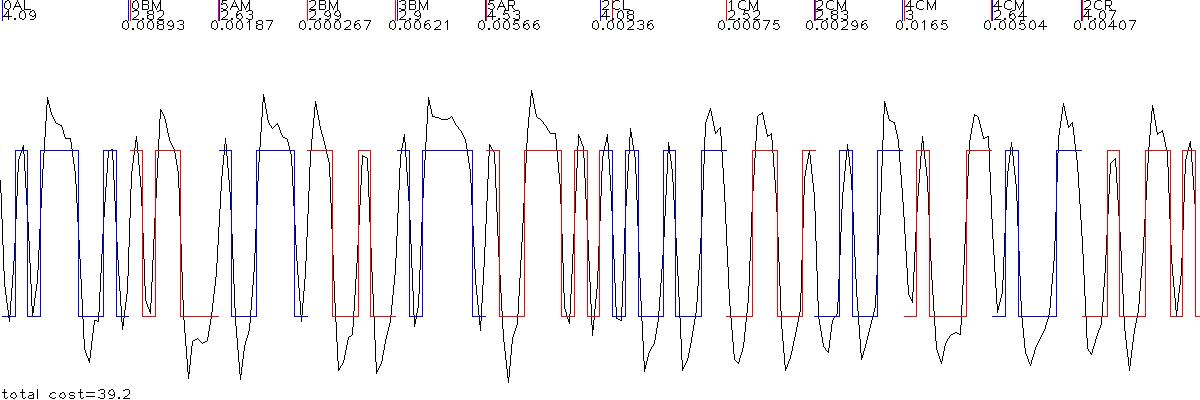
\includegraphics[width=\textwidth,natwidth=1200,natheight=400]{img/tmpl.jpg}
\caption{Successful reading with template matching. Templates shown in red and blue.}
\label{tmpl}
\end{figure}





% Let $S=\set{0A, 1A,\cdots 9A, 0B, \cdots, 9C}$ be the set of possible patterns.
% A base template for the pattern $s\in S$ is a function $\mm^s(x)$ as shown in
% FIGGGGGURE. The patterns from the EAN-13 standard are augmented by one bar of
% the The deformed template has been shifted by an offset $o$ and scaled
% by a base width $w$:
% \begin{equation*}
%  \mm^s_{o,w} (x)=\mm^s((x-o)/w)
% \end{equation*}
% For each position in the barcode and conditioned on a specific choice of $o$ and $w$, we
% can calculate the matching probability for a pattern $s\in S$ as
% \begin{equation*}
%  p_s(I\mid o,w) \propto e^{-D(I, \mm^s_{o,w})}\,,
% \end{equation*}
% where $I(n)$ represents the grey values of the current scanline. $D$ is a
% distance measure between the template and the scanline and is calculated
% pixel by pixel:
% \begin{equation*}
%   D(I, \mm^s_{o,w}) = \sum_{n=}
% \end{equation*}

%%% Local Variables:
%%% mode: latex
%%% TeX-master: "00Ausarbeitung.tex"
%%% End:
 
\newpage

\section{Vergleich} 
\subsection{Pros and Cons}\label{sec:ProCon}
\subsubsection*{Gradient + Blur}
Pros:

Gradien+Blur is conceptually extremely simple and therefore extremely fast. It also is robust against disturbances like reflections since it only looks for the biggest contour.
\\
\\
Cons:

Since the algorithm uses the absolute gradient difference it is quite weak against rotations of 45 degrees. Gradient+Blur is also dependent on many parameters. If these parameters don't match up with the barcode the algorithm fails. One such instance is a too small kernel size for the closing step, which leads to a fragmented contour because it fails to close the white segments. An example of this can be seen in \cref{failgradblur}. Another problem is the susceptibility to noise. Gradient+Blur could mistake the wrong contour for the barcode.

\begin{figure}[t]
\center

\includegraphics[width=0.4\textwidth,natwidth=800,natheight=600]{img/gradientblurfail.jpg}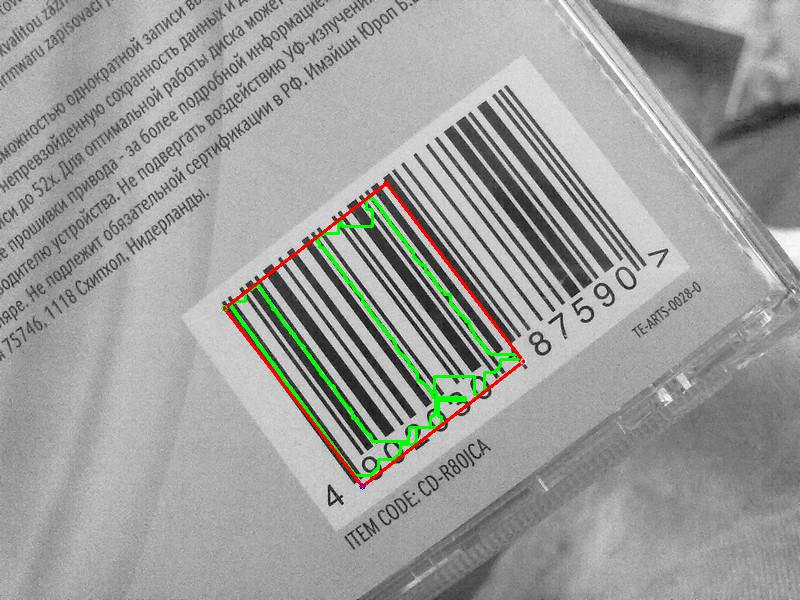
\includegraphics[width=0.4\textwidth,natwidth=800,natheight=600]{img/gradientblurfail2.jpg}
\caption{If the kernel size does not match to the barcode size Gradient+Blur fails to fully close the contour. The detected barcode is shown in red.}
\label{failgradblur}
\end{figure}

\subsubsection*{LSD}
Pros:

The LSD is still relatively fast and can reliably detect a barcode in almost every position and rotation.
\\
\\
Cons:

The LSD looks for all parallel lines. If there are textures in the image with a
large number of parallel lines, these could be mistaken for a barcode. Disturbances like reflections can also break barcode lines and lead to exclusion valid lines.

\subsubsection*{Variation}
Pros:

The variation boundary finder is not dependent on the line segments returned by
LSD, so that good boundaries can still be found even if the LSD result is bad
due to glare spots, bad focus, etc. 
\\
\\
Cons:

Structures with large variation next to the barcode, such as text, can result in the boundaries
being extended beyond the barcode. Additionally, the bars of the outer guard
patterns are very thin and may not result in enough variation, especially if
there is some amount of blur. The variation boundary finder will tend to cut off
the last few bars on each side.

\subsubsection*{LSD Bound}
Pros:

Because of the high quality of line segments returned by LSD, this method is
very good at accurately determining the boundary segments. We return
multiple candidates on each side, so that some variance can be dealt with.
\\
\\
Cons:

Since it is strongly dependent on the LSD localization it fails as soon as the LSD localization fails. And since an enormous amount of lines needs to be tested the algorithms is not suited for real time applications.

\subsubsection*{Wachenfeld}
Pros:

The Wachenfeld algorithm is relatively quick since it is based on a scanline.
\\
\\
Cons:

The algorithm is strongly dependent on the quality of the preprocessing and detection of local extrema. And since the algorithm is based on a scanline it has no way to deal with broken barcodes caused by disturbances as seen in \cref{failwachenfeld}. Finally, if the last segment selection steps misses, the barcode can be shifted to the left or right and become unreadable.

\begin{figure}[t]
\center

\includegraphics[width=0.4\textwidth,natwidth=800,natheight=600]{img/wachenfeldfail.jpg}
\hspace{1cm}
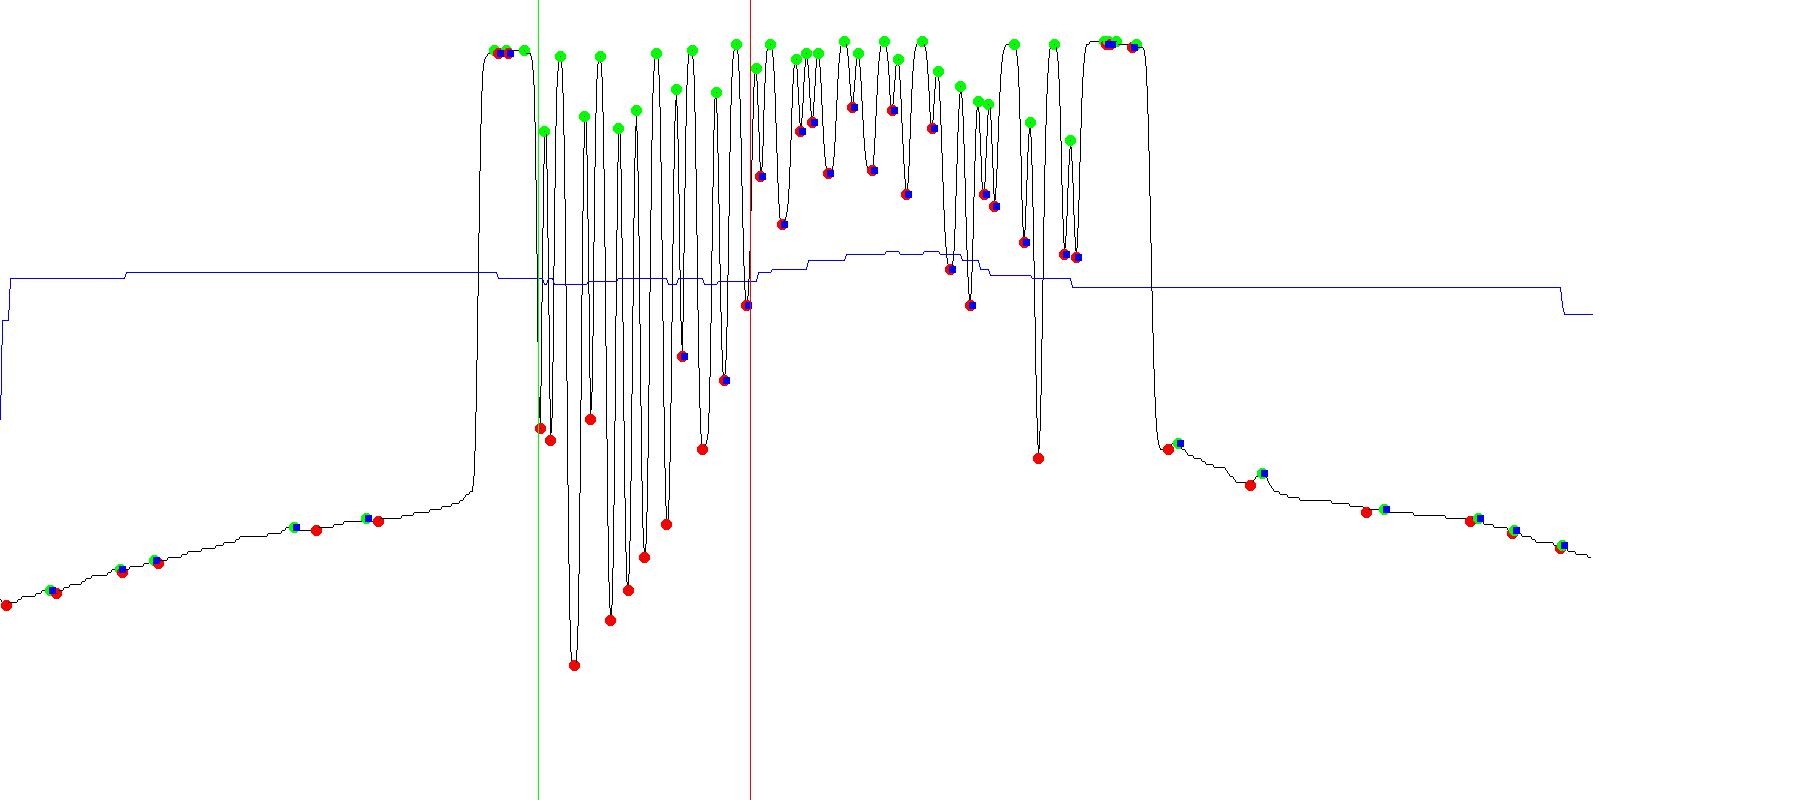
\includegraphics[width=0.5\textwidth,natwidth=1800,natheight=800]{img/wachenfeldfail2.jpg}
\caption{Preprocessin failing to apply dynamic thresholding and determining local extrema because of light reflections.}
\label{failwachenfeld}
\end{figure}
 
\subsubsection*{Template Matching}
Pros:

Since no binarization is required, template matching is extremely robust against
blurred barcodes. Some uncertainty in the localization and boundary detection
can be dealt with.
\\
\\
Cons:

The matching process required precomputed data to be matched against the barcode. This can take a lot of time and memory depending on the targeted accuracy. And since the template matching is based on probability it is more likely to return a false positive result than no result.
\vfill %nur für die abagabe für ein besseres layout
\subsection{Datasets}
The implemented algorithms were tested on three datasets.
\begin{itemize}
\item Generated Barcodes:
\begin{itemize}
\item 110 images, 300$\times$150 px, barcode only.
\item 110 images, 1000$\times$1000 px, barcodes (300$\times$150 px) randomly rotated and translated on white background.
\end{itemize}
\item WWU Muenster Barcode Database \cite{MuensterBarcodeDB} \citep{wachenfeld2008robust}:\\
1055 images, 800$\times$600 px.
\item ArteLab Dataset - Robust Angle Invariant 1D Barcode Detection \cite{ArteLabDB} \cite{zamberletti2010neural} \citep{zamberletti2013robust}:\\
2 sets of 215 images, 800$\times$600 px.
\end{itemize}

\subsection{Run time and Accuracy Comparison}
The algorithms were compared over the 1055 images of the WWU Muenster Barcode Database \citep{MuensterBarcodeDB}. The programm was implemented in C++ with the help of the Qt 5.7 and OpenCV 3.1 frameworks. The test were made on a Debian 8 system with an Intel N2940 CPU, 4 Cores / 4 Threads, and 4 GB RAM. The results are shown in \cref{laufzeit}.
\\
\\
The experimental results illustrate the pros and cons of the various algorithms
shown in \cref{sec:ProCon}. The Gradient+Blur algorithm performs the best in
respect to speed but the worst in respect to accuracy. The simplicity of the
method is directly apparent, but the listed problems cause it to miss the boundaries or even fail to detect the barcode.

The second fastest algorithm is the Wachenfeld boundary detection. This is
primary achieved through the usage of a single scanline. But the unoptimized
preprocessing causes the algorithm to miss the boundaries in over 40\% of tests
since the dynamic thresholding fails to accurately binarize the scanline.

Both Variation Boundary Detection and LSDBounds take a very long time. This is caused by the multiple computation heavy probings of
possible boundaries, which results in 126 different scanlines being read for
each barcode. However, this allows a correct barcode to be read even if some
boundary detections are invalid, which results in a high accuracy.


\begin{figure}[t]
\center
\bgroup
\def\arraystretch{1.5}
\begin{tabular}{|l|r|r|r|}
\hline
&\textbf{Errors}&\textbf{Accuracy}&\textbf{Time in sec.}\\
\hline
\textbf{Gradient + Blur}& 831& 22\%& 266\\
\hline
\textbf{LSD + Variation}& 279& 74\%& 1595\\
\hline
\textbf{LSD + LSDBounds}& 41& 97\%& 1760\\
\hline
\textbf{LSD + Wachenfeld}& 452& 56\%& 319\\
\hline
\end{tabular}
\egroup
\caption{Comparison of different algorithms on the WWU Muenster Barcode Database. All algorithms use Template Matching to read the barcode.}
\label{laufzeit}
\end{figure}
 
%%% Local Variables:
%%% mode: latex
%%% TeX-master: "00Ausarbeitung.tex"
%%% End:
\newpage

\section{Verbesserung} 
In this section, we will consider some possible improvements to our implementation of the algorithms.

\subsection{Gradient+Blur Detection}

\subsubsection*{Vary by rotation}
Since the Gradient+Blur-detection builds from the absolute gradients found by the Sobel operator, results might be poor when a barcode is rotated close to 45 degrees. To remedy this, we might run the detection on rotated versions of the image. Rotating once by 45 degrees would yield the greatest improvement, however, multiple rotations could be checked at diminishing returns.

\subsubsection*{Vary kernel sizes}
In our current implementation, all operations (blurring, closing, opening) are applied with a constant kernel size. This is somewhat problematic, since the effectiveness of these parameters is dependent on the size of the barcode. If a barcode is not detected successfully, we might try different kernel sizes.\newline
The initial kernel size might also be considered further: The current values have been empirically determined to be most useful for the image sizes we worked with. Scaling the kernel size appropriately for each image might lead to better results, since it seems likely that the relative sizes barcodes in images is independent of image resolution.


\subsection{LSD}
\subsubsection*{Unite interrupted line segments}

A remaining common failure of the LSD algorithm is it's poor handling of reflections on the barcode. These reflections visually interrupt the barcode lines, so two short line segments are returned instead of one. This is problematic, as length of line segments is an important factor in deciding whether two line segments might be part of the same barcode. This ultimately leads to a split in the barcode, where the detected area covers just the larger side of the code.

This problem could be fixed in two related ways: First, we could try a \emph{line segment unification}. This process would seek to unite line segments which lie on the same line in space. This easy calculation would unite line segments across gaps, thus restoring the proper length and avoiding rejection. To avoid uniting many stray lines across the image, simply limit unification to line segments where the gap size is less than some small multiple of the segment size itself.

This first approach has the weakness of only working when the reflection splits the line segment into two parts. Even better would be an approach that could handle a missing endpoint. This should be handled by this second approach, which is also more complicated: Instead of uniting line segments, we would now consider the endpoints of line segments in a second pass over all segments. During the first pass, whenever a pair of lines is considered to likely be part of the same barcode, save the location of their endpoints in two different lists, based on distance from the origin. After this first pass, those lists can easily construct the upper and lower bound of the barcode. With this new information, discard the previous scores and redo them. However, this time, instead of checking for similar length, check whether two line segments have an endpoint near one of those two lines before assigning a score to them. This second pass will now also handle missing endpoints.

\subsection{Wachenfeld}
\subsubsection*{Proper preprocessing, multiple scanlines}

Since we have found quick success with the LSD-Boundary detection, our current implementation of the Wachenfeld algorithm does not prepare the image in the way recommended in the original paper, that is, there is no adaptive thresholding along the scanline, which is a major factor of success for the original implementation. Thus, proper initialization would likely greatly improve our results. Also, we could detect along multiple scanlines and vote for most likely boundaries.

\subsection{Template Matching}
\subsubsection*{Precompute patterns for blur of various strengths}

While the algorithm is already very capable in handling blurred barcodes, this might be improved even further by precomputing patterns specifically not for an ideal, clean barcode, but for one that is already blurred.

\newpage

\section{Fazit} 
In this work we have seen how different algorithms compare against each other in detecting barcodes.

After some initial comparisons of Gradient+Blur and LSD we decided to go with the latter because of the superior localization quality. And since we were satisfied with the high quality of the readings performed by the Template Matching we decided to focus our efforts on improving the overall hit rate by implementing additional boundary detection algorithms.

While comparing the Wachenfeld boundary detection against the Variation boundary detection we have shown that by sacrificing speed and increasing complexity we can increase the detection rate. Since we wanted to maximize the overall hit rate with regards to the competition within the scope of the practical course we improved on the Variation boundary detector by sacrificing more time and resources in favor of the LSDBound algorithm.

Obviously our methodology is not applicable for real time usage in the wild. A more fitting approach would be to implement a fast and simple algorithm like gradient blur enhanced with additional scan line based refinement like the Wachenfeld algorithm with optimized preprocessing and reading step. In a real time application the algorithm could depend on the user to provide sharp and disturbance free images with centered barcodes without rotation. 
\\
\\
Finally our work can be summarized with: Higher accuracy detection and recognition of barcodes in a non-constrained system takes more time and resources.
\newpage


\section{Meta: Wie zitiere ich?} 
\begin{enumerate}
\item Titel des Papers bei \url{https://scholar.google.de/} Google Scholar suchen.
\item Bei dem Eintrag zu dem Paper unten auf zitieren klicken, dann auf BibTex.
\item Den BibTex string kopieren in die \textsc{literatur.bib}
\item Zitat hinzufügen durch \textsc{\textbackslash cite\{\textit{name}\}}
\item Übersicht BibTex: \url{https://de.wikibooks.org/wiki/LaTeX-Kompendium:_Zitieren_mit_BibTeX}
\end{enumerate}
Beispiel Templatematching \cite{chen2014scanning}
%\input{03titel}

Einleitung
Lokalisierung
Rand
Lesen
Testdaten
Vergleich der Verfahren
Verbesserung



%\newpage
%\section{Einleitung} 
%\input{04titel}

\newpage
\appendix
\printbibliography
\end{document}
